\documentclass[journal]{IEEEtran}

\ifCLASSINFOpdf
\usepackage[pdftex]{graphicx}
  % declare the path(s) where your graphic files are
  % \graphicspath{{../pdf/}{../jpeg/}}
  % and their extensions so you won't have to specify these with
  % every instance of \includegraphics
\DeclareGraphicsExtensions{.pdf,.jpg,.png}
\else
  % or other class option (dvipsone, dvipdf, if not using dvips). graphicx
  % will default to the driver specified in the system graphics.cfg if no
  % driver is specified.
  % \usepackage[dvips]{graphicx}
  % declare the path(s) where your graphic files are
  % \graphicspath{{../eps/}}
  % and their extensions so you won't have to specify these with
  % every instance of \includegraphics
  % \DeclareGraphicsExtensions{.eps}
\fi

\begin{document}

\title{Fast, Distributed Data-Graph Computation for Physical Simulation}

\author{James~Thomas% <-this % stops a space
}


% The paper headers
%\markboth{Thomas}

\maketitle

% As a general rule, do not put math, special symbols or citations
% in the abstract or keywords.
\begin{abstract}
We investigate the problem of executing physical simulations efficiently on a cluster of computers. We cast the problem as a data-graph computation in the style of GraphLab, where vertices represent points in a physical mesh and edges connect nearby vertices. Taking advantage of the special properties of mesh graphs, including the locality of edges, we devise and evaluate schemes for partioning such graphs across a cluster of computers to minimize communication and for performing vertex updates on individual machines with high cache locality and parallelism.
\end{abstract}

% Note that keywords are not normally used for peerreview papers.

\IEEEpeerreviewmaketitle



\section{Introduction}
The age of big data is upon us. Organizations large and small are coping with massive volumes of data from sensors, website clicks, e-commerce, and more. In recent years, there has been growing
interest in developing frameworks for the storage and analysis of this data on large compute clusters. Hadoop \cite{hadoop} has been among the most popular of these. It breaks up large datasets into small pieces spread across a cluster and then allows users to supply computations (maps) that are run over the pieces independently and then computations (reduces) that combine the results. Many problems can be cast into the Hadoop model, but in many cases the Hadoop approach is far less effecient than more specialized methods.

Iterative graph algorithms are one class of problems where Hadoop leaves a lot to be desired. In particular, each Hadoop computation writes its output to disk, so each iteration in iterative computations incurs the overhead of a disk write and then a subsequent disk risk for the next iteration. In addition, graphs are difficult to split into completely independent sets (with no crossing edges) for the map phase of a Hadoop computation, so the maps are often wasteful.

In response to these shortcomings of Hadoop and similar systems, Carlos Guestrin and his collaborators developed the GraphLab platform \cite{graphlab} for iterative graph algorithms. The computation model here associates data with each node in a graph, and in each iteration runs an update function on each node that takes as input the data of the node and that of its neighbors. A node can only be updated for the $n$th time if its neighbors have been updated either $n-1$ or $n$ times. Many interesting big data algorithms, including Google's PageRank, can be easily expressed under this model. GraphLab comes in two variants -- a single-machine implementation that attains parallelism by updating nodes concurrently on multiple processing cores, and a distributed implementation that additionally spreads vertices across machines.

As GraphLab and competing frameworks have become more popular, there has been growing interest in optimizing their execution. In the single-machine case, there has been work on reducing costly sychronization steps and more generally on increasing parallelism so that performance can scale up as core counts grow. In the distributed case, the single-machine optimizations have been supplemented by work on more effectively splitting up nodes into sets with few crossing edges so that expensive inter-machine communication can be reduced.

\begin{figure}[!t]
\centering
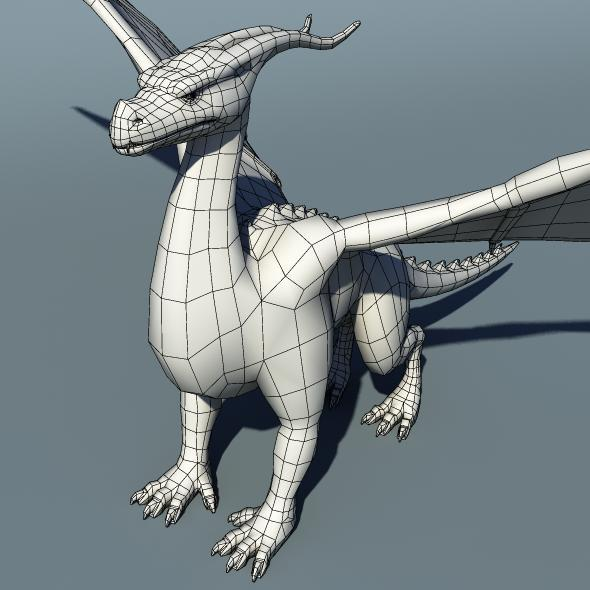
\includegraphics[width=2.5in]{dragon}
\caption{A mesh graph where lines correspond to edges and intersections of lines correspond to vertices.}
\label{fig_mesh}
\end{figure}

In this work, we optimize a graph processing framework for a specific workload: physical mesh simulations. A mesh graph is embeddable in 3D space, and an example is shown in Figure 1. Mesh graphs have the nice property that we can partition them into sets corresponding to arbitrary contiguous regions in physical space, and edges cross out of a particular set only from vertices near the boundaries of its physical region. Thus, the number of edges crossing out of a set is proportional to the surface area of its physical region, which is a fairly small quantity relative to the number of vertices, especially when the region has large volume.

Taking advantage of these properties, we use a novel method based on space-filling curves to split up an input mesh graph across machines to limit inter-machine communication. We then optimize performance on individual machines by evaluating a number of techniques for the scheduling of vertex updates that hit different points in the cache/TLB locality and parallelism design space. Some of our results yield insights for more general classes of graphs.

% Discussion of BSP vs. Gauss-Siedel?

\section{Dealing with Distributed Execution}
Since an update function can only be run on a vertex if its neighbors are at most one iteration behind, we need to incur network traffic on every iteration to communicate vertex values for edges that cross machines. This can be done in a few ways. First, when an update function is being run on a vertex, it can fetch the values for neighbors on different machines and then run the necessary computation. This synchronous approach seems less than ideal, since the network traffic falls on the critical path of the iteration -- it is very likely that vertices that are capable of being updated without any network requests are waiting idle as the network requests complete.

Thus, an asynchronous approach is generally preferable. Our approach is as follows. For each edge that crosses machines, we declare one endpoint vertex as the predecessor and the other as the successor. Once the predecessor is updated, it sends its value to the machine to which the successor is assigned. Once the successor has received values from all of its predecessors, it can be scheduled for execution. If our partioning of vertices across machines is good and there are many vertices on each machine that have no dependencies on external vertices and therefore can be scheduled at any time, then there will be minimal waiting for network messages. Our scheme ensures that we satisfy the constraint that vertex updates must appear to be processed in some global order -- in other words, both of the endpoints of an edge cannot be updated in some iteration based on the other's data from the previous iteration.

\begin{figure}[!t]
\centering
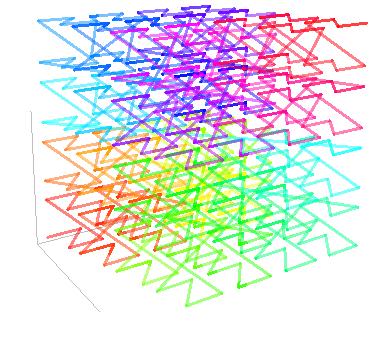
\includegraphics[width=2.5in]{z}
\caption{A Z-order curve tracing out the 3D space bounded by the box.}
\label{fig_z}
\end{figure}

We partition vertices across machines using a technique based on space-filling curves. A 3D space-filling curve maps the real numbers to points in 3D space so that for an arbitrary point $p$ as we trace out more and more of the curve the distance from $p$ to the nearest point on the curve becomes smaller and smaller. We use a Z-order curve, which has the property that if two points on the curve are relatively close together, then the real numbers that generated those points tend to be relatively close. A Z-order curve in 3D space is shown in Figure 2.

Each vertex in a mesh graph can be assigned a particular coordinate in 3D space. Thus, we can draw a bounding box in 3D space around a mesh graph. We trace out a Z-order curve over a finite portion of its domain mapping to points in the bounding box. We then assign each vertex in the mesh to its nearest point in the traced curve and mark the vertex with the real number that generated this point, which we will call the Z-number. We then sort the vertices by Z-number. Nearby vertices in the sorted order should be nearby in the physical graph. We can then split this sorted list into contiguous chunks, one for each machine in our cluster. Since each chunk should correspond to some contiguous region in 3D space, the number of edges crossing machines should be fairly small, as explained in the previous section.

\section{Fast Execution on Individual Machines}

Once we have a good vertex partitioning and a strategy for distributed execution, throughput depends largely on single-machine performance. We explore a number of schemes to this end.

\begin{figure*}[ht]
\centering
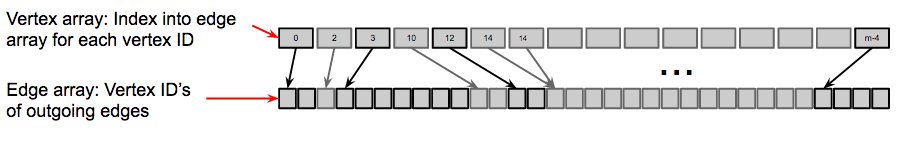
\includegraphics[width=\textwidth,keepaspectratio]{layout}
\caption{Organization of graphs in memory on a single machine.}
\label{fig_layout}
\end{figure*}

\subsection{Graph Representation in Memory}
We represent graphs in memory on a single machine as follows. We have an array of vertices and an array of edges. Each vertex contains data and a pointer into the edge array indicating the start of its list of edges. Adjacent vertices have adjacent edge lists. Each edge is simply a pointer into the vertex array. This organization is shown in Figure 3.

\subsection{Scheduling for Parallel Execution}
There are two major strategies for scheduling vertices for parallel execution that preserve the appearance of a global ordering across updates and avoid data races. The first is coloring \cite{chromatic}. If we color a graph so that no two neighboring vertices have the same color, we can safely execute the updates for vertices of the same color in fully in parallel. The reason is that if any vertex's data is being written by some thread, it cannot be read in parallel by another thread because this would require a neighbor of this vertex to be updating concurrently, which is impossible. With the coloring strategy, we sort the vertex array (and the corresponding edge lists) by color and step sequentially through the colors, updating the vertices of each color in a parallel loop.

The other strategy is priority DAG scheduling \cite{dag}. This involves assigning each vertex a distinct priority, so that we can form a DAG from our graph by adding a direction to each edge such that the source is the endpoint vertex with higher priority. We assign each vertex a counter equal to the number of predcessors it has. We can start by executing all vertices with no predecessors in parallel. Once a vertex is complete, we atomically decrement the counter of each of its successors. If a vertex's counter becomes zero, we can spawn the update of this vertex as another parallel strand of execution. We thus attain fairly high parallelism at the cost of using atomics, which can involve expensive memory barriers on modern hardware. Once again, there can be no data races because two neighboring vertices cannot execute concurrently since one must be the predecessor of the other.

\subsection{Achieving Cache Locality}
If we update the vertices in the vertex array sequentially, as we do with coloring-based scheduling, we get good cache locality (cached lines are processed completely after being fetched) on our accesses to the vertices being updated and to their corresponding entries in the edge array, which is also processed sequentially. Cache locality here includes data cache and TLB locality, since pages in the vertex and edge arrays corresponding to vertices being updated are processed completely after their first access. TLB misses have been shown to be a significant factor in the runtimes of data-intensive computations and are an important consideration for us.

While we get good locality on edge and vertex array accesses for vertices being updated, we get poor locality for accesses to the vertex array to fetch these vertices' neighbors. These accesses are essentially random unless we have sorted the vertex array in some locality-improving manner. Ideally we could store vertices' neighbors close to them in the vertex array. This would confer two benefits. First, TLB misses would fall since neighbors of a vertex will in most cases be stored in the same page as the vertex. Secondly, if a vertex being updated pulled neighbors that were yet to be updated into cache, those neighbors would be updated before they left cache, reducing cache misses.

These considerations suggest that ordering vertices in the vertex array by breadth-first search (BFS) level would be helpful. A vertex at BFS level $n$ can only have neighbors at BFS levels $n-1$ and $n+1$; if there was a neighbor at a smaller level, the vertex would have smaller level than $n$, and there can be no neighbors at levels greater than $n+1$ if the vertex is at $n$. Thus, if BFS levels are fairly small, ordering the vertices by BFS level would result in nearby neighbor accesses as desired. BFS levels are generally bounded in size in mesh graphs; they grow at first, but once the largest cross-section of the mesh is reached, successive levels should have similar size. The problem with ordering the entire vertex array by BFS level is that there are no longer defined sequential regions over which parallel update loops can be run -- since any two adjacent vertices could be neighbors -- so parallelism is lost. We implement and evaluate a hybrid coloring-BFS approach that restores some parallelism while preserving our locality wins: within each BFS level, we sort by color, so that within each BFS level we can update the vertices of each color in parallel. The BFS levels are executed sequentially. This scheme brings up an important point about the locality-parallelism design space -- after a point, increasing parallelism is not necessarily important. If there is enough parallelism to saturate the cores of the available machines, locality is likely the parameter worth optimizing.

% Analyze for priority DAG case
In the case of priority DAG scheduling, cache behavior is very different. We lose the locality of access to the vertex and edge arrays for vertices being updated that we have in the sequential processing case. But we are not without victories: when we update the last predecessor of some node we immediately afterwards update that node, at which point is hot in cache. So accesses to neighbors of vertices being updated do not have worst-case cache behavior as they do in the sequential processing case.

For ideal cache behavior, the story is similar to the sequential processing case. We would like for neighborhoods of nearby vertices to be stored fairly contiguously in the vertex array so that accesses to neighbors of vertices being updated tend not to cause TLB misses. We would also like these neighborhoods to be updated completely in some small time window so that fetched neighbors are updated before they leave cache. Achieving the first objective is possible by using a BFS-based ordering or by preserving the Z-number ordering described above for partitioning vertices across machines. We take the second approach because BFS levels may be larger than memory pages and therefore TLB misses are more likely under the BFS-based ordering. Achieving the second objective is much harder with DAG scheduling because the order in which vertices are updated is unclear. However, if we assign each vertex a priority equal to its Z-number, we suspect that if we spawn off the processing of vertices with no predecssors in order of Z-number and if we can assume that earlier spawned routines tend to execute to completion before later spawned routines begin executing (as is the case in the Cilk model of multithreading), then contiguous regions of the physical mesh should be processed nearly to completion in small periods of time. 

% "small period of time" is not precise...

%Draw parallel to cache-oblivious?

\subsection{Considering Parallelism}
% atomics, barriers in the priority DAG case
% cache transfers across processors are fast -- so as long as the data is in some cache, we are OK (not for TLB though) ... BUT
% Cilk -- steals high in the tree

\subsection{Prefetching}


\ifCLASSOPTIONcaptionsoff
  \newpage
\fi

\begin{thebibliography}{1}

\bibitem{graphlab}
Y.~Low et. al. \emph{GraphLab: A New Framework for Parallel Machine Learning}. \it{UAI}, 2010.

\bibitem{hadoop} 
\emph{Hadoop}. http://hadoop.apache.org. 2015.

\bibitem{dag}
W.~Hasenplaugh et. al. \emph{Ordering Heuristics for Parallel Graph Coloring}. \it{SPAA}, 2014.

\bibitem{chromatic}
T.~Kaler et. al. \emph{Executing Dynamic Data-Graph Computations Deterministically Using Chromatic Scheduling}. \it{SPAA}, 2014.

\end{thebibliography}

\end{document}


